\section{Finding Limits Analytically}\label{sec:limit_analytically}

In \autoref{sec:limit_intro} we explored the concept of the limit without a strict definition, meaning we could only make approximations. In the previous section we gave the definition of the limit and demonstrated how to use it to verify our approximations were correct. Thus far, our method of finding a limit is (1) make a really good approximation either graphically or numerically, and (2) verify our approximation is correct using an $\epsilon$-$\delta$ proof.

Recognizing that $\epsilon$-$\delta$ proofs are cumbersome, this section gives a series of theorems which allow us to find limits much more quickly and intuitively. \bigskip

Suppose that $\ds\lim_{x\to 2} f(x)=2$ and $\ds\lim_{x\to 2} g(x) = 3$. What is $\ds\lim_{x\to 2}(f(x)+g(x))$? Intuition tells us that the limit should be 5, as we expect limits to behave in a nice way. The following theorem states that already established limits do behave nicely.

\theorem{thm:limit_algebra}{Basic Limit Properties}{%
Let $b$, $c$, $L$ and $K$ be real numbers, let $n$ be a positive integer, and let $f$ and $g$ be functions with the following limits: \index{limit!properties}
$$\lim_{x\to c}f(x) = L \text{\ and\ } \lim_{x\to c} g(x) = K.$$
The following limits hold.
\begin{enumerate}
\item	\makebox[9em][l]{Constants:} $\ds\lim_{x\to c} b = b$
\item	\makebox[9em][l]{Identity:} $\ds\lim_{x\to c} x = c$
\item	\makebox[9em][l]{Sums/Differences:} $\ds\lim_{x\to c}(f(x)\pm g(x)) = L\pm K$
\item	\makebox[9em][l]{Scalar Multiples:}	$\ds\lim_{x\to c} b\cdot f(x) = bL$
\item	\makebox[9em][l]{Products:}	$\ds\lim_{x\to c} f(x)\cdot g(x) = LK$
\item	\makebox[9em][l]{Quotients:} $\ds\lim_{x\to c} f(x)/g(x) = L/K$, ($K\neq 0$)
\item	\makebox[9em][l]{Powers:} 	$\ds\lim_{x\to c} [f(x)]^n = L^n$
\item	\makebox[9em][l]{Roots:} $\ds\lim_{x\to c} \sqrt[n]{f(x)} = \sqrt[n]{L}$ \quad {\small (when $n$ is odd or $L\ge0$)}
\end{enumerate}}

We will now prove the Sum Property using the formal definition of a limit from the previous section. We know that $\ds \lim_{x\to c}f(x) = L$ and  $\ds\lim_{x\to c} g(x) = K$. We want to show that $\ds \lim_{x\to c}f(x)+g(x)=L+K$.

\begin{proof}
We must show that given any $\epsilon>0$, we can find a $\delta>0$ such that
\[\text{if }0<\abs{x-c}<\delta,\text{ then }\abs{f(x)+g(x)-(L+K)}<\epsilon.\]
We know $\ds \lim_{x\to c}f(x) = L$. So for any $\epsilon_1 >0$, we can find $\delta_1>0$ such that if $0<\abs{x-c}<\delta_1$, then $\abs{f(x)-L}<\epsilon_1$. Similarly we know $\ds\lim_{x\to c} g(x) = K$ so for any $\epsilon_2>0$, we can find $\delta_2>0$ such that if  $0<\abs{x-c}<\delta_2$, then $\abs{g(x)-K}<\epsilon_2$. We will let both $\epsilon_1$ and $\epsilon_2$ be $\frac{\epsilon}{2}$. Now, we have a $\delta_1>0$ and a $\delta_2>0$ such that:
\begin{gather*}
\text{if }0<\abs{x-c}<\delta_1,\text{ then }\abs{f(x)-L}<\frac{\epsilon}{2} \\
\text{and} \\
\text{if }0<\abs{x-c}<\delta_2,\text{ then }\abs{g(x)-K}<\frac{\epsilon}{2}
\end{gather*}
We will choose $\delta=\min(\delta_1,\delta_2)>0$. If $0<\abs{x-c}<\delta$, then $\abs{f(x)-L}<\frac{\epsilon}{2}$ and  $\abs{g(x)-K}<\frac{\epsilon}{2}$.  Add the two inequalities together so that
\[\abs{f(x)-L}+\abs{g(x)-K}<\frac{\epsilon}{2}+\frac{\epsilon}{2}=\epsilon.\]
We will now use the triangle inequality: $\abs{A+B}\leq\abs{A}+\abs{B}$.
\[\abs{f(x)-L+g(x)-K}\leq\abs{f(x)-L}+\abs{g(x)-K}<\epsilon\]
Thus $\abs{(f(x)+g(x))-(L+K)}<\epsilon$, which is what we were trying to show.
\end{proof}

The other Basic Limit Properties can be proven in a similar way and are left for the reader.  Our next theorem requires a few more conditions.

\theorem{thm:limit_composition}{Limits of Composition}{Suppose that
\[\lim_{x\to c}f(x)=L\text{ and }\lim_{x\to L}g(x)=g(L)=K.\]
Then $\ds\lim_{x\to c}g(f(x))=K$.}
% continuity of g required: f=g=1_{x==0} so f(g)=1_{x!=0}

\youtubeVideo{v_Nz6UUQ4HQ}{Limit Laws to Evaluate a Limit, Example 1}

We apply the theorem to an example.

\example{ex_basic_limit_1}{Using basic limit properties}{Let
\[
 \lim_{x\to 2} f(x)=2,\quad\lim_{x\to 2} g(x) = 3\qquad\text{and}\qquad
 p(x) = 3x^2-5x+7.
\]
Find the following limits:\\
\begin{minipage}[t]{.5\textwidth}
\begin{enumerate}
	\item	$\ds \lim_{x\to 2} \big(f(x) + g(x)\big)$
	\item	$\ds \lim_{x\to 2} \big(5f(x) + g(x)^2\big)$
\end{enumerate}
\end{minipage}%
\begin{minipage}[t]{.5\textwidth}
\begin{enumerate}\addtocounter{enumi}{2}
	\item	$\ds \lim_{x\to 2} p(x)$
\end{enumerate}
\end{minipage}}
{\begin{enumerate}
	\item	Using the Sum/Difference rule, we know that $\ds \lim_{x\to 2} \big(f(x) + g(x)\big) = 2+3 =5$.
	\item	Using the Scalar Multiple and Sum/Difference rules, we find that\\ $\ds \lim_{x\to 2} \big(5f(x) + g(x)^2\big) = 5\cdot 2 + 3^2 = 19.$
	\item	Here we combine the Power, Scalar Multiple, Sum/Difference and Constant Rules. We show quite a few steps, but in general these can be omitted:
	\begin{align*}
		\lim_{x\to 2} p(x) &= \lim_{x\to 2} (3x^2-5x+7) \\
		&= \lim_{x\to 2} 3x^2-\lim_{x\to 2} 5x+\lim_{x\to 2}7 \\
		&= 3\cdot 2^2 - 5\cdot 2+7 \\
		&= 9.\eoehere
	\end{align*}
\end{enumerate}}

Part 3 of the previous example demonstrates how the limit of a quadratic polynomial can be determined using the properties of \autoref{thm:limit_algebra}. Not only that, recognize that $$\lim_{x\to 2} p(x) = 9 = p(2);$$ i.e., the limit at 2 was found just by plugging 2 into the function. This holds true for all polynomials, and also for rational functions (which are quotients of polynomials), as stated in the following theorem.

\theorem{thm:poly_rat}{Limits of Polynomial and Rational Functions}{Let $p(x)$ and $q(x)$ be polynomials and $c$ a real number. Then:
\begin{enumerate}
\item	$\ds \lim_{x\to c} p(x) = p(c)$
\item	$\ds \lim_{x\to c} \frac{p(x)}{q(x)} = \frac{p(c)}{q(c)}$, where $q(c) \neq 0$.
\end{enumerate}
}

\example{ex_limit_rat}{Finding a limit of a rational function}{Using \autoref{thm:poly_rat}, find $$\lim_{x\to -1} \frac{3x^2-5x+1}{x^4-x^2+3}.$$}
{Using \autoref{thm:poly_rat}, we can quickly state that 
	\begin{align*}
		\lim_{x\to -1}\frac{3x^2-5x+1}{x^4-x^2+3}
		&= \frac{3(-1)^2-5(-1)+1}{(-1)^4-(-1)^2+3} \\
		&= \frac{9}{3} =3.\eoehere
	\end{align*}}

It was likely frustrating in \autoref{sec:limit_def} to do a lot of work to prove that $$\lim_{x\to 2} x^2 = 4$$ as it seemed fairly obvious. The previous theorems state that many functions behave in such an ``obvious'' fashion, as demonstrated by the rational function in \autoref{ex_limit_rat}. 

Polynomial and rational functions are not the only functions to behave in such a predictable way. The following theorem gives a list of functions whose behavior is particularly ``nice'' in terms of limits. In the next section, we will give a formal name to these functions that behave ``nicely.''

\ifthenelse{\boolean{longpage}}{}{\setboxwidth{100pt}}
\theorem{thm:lim_continuous}{Limits of Basic Functions}{%
Let $c$ be a real number in the domain of the given function and let $n$ be a positive integer. The following limits hold:\\
\begin{minipage}[t]{.33\specialboxlength}
\begin{enumerate}
\item		$\ds \lim_{x\to c} \sin x = \sin c$
\item		$\ds \lim_{x\to c} \cos x = \cos c$
\item		$\ds \lim_{x\to c} \tan x = \tan c$
\end{enumerate}
\end{minipage}%
\begin{minipage}[t]{.33\specialboxlength}
\begin{enumerate}\addtocounter{enumi}{3}
\item		$\ds \lim_{x\to c} \csc x = \csc c$
\item		$\ds \lim_{x\to c} \sec x = \sec c$
\item		$\ds \lim_{x\to c} \cot x = \cot c$
\end{enumerate}
\end{minipage}%
\begin{minipage}[t]{.33\specialboxlength}
\begin{enumerate}\addtocounter{enumi}{6}
\item		$\ds \lim_{x\to c} a^x = a^c$ ($a>0$)
\item		$\ds \lim_{x\to c} \ln x = \ln c$
\item		$\ds \lim_{x\to c} \sqrt[n]{x} = \sqrt[n]{c}$
\end{enumerate}
\end{minipage}}

Many times, we will combine this theorem with Theorems \ref{thm:limit_algebra} and \ref{thm:limit_composition}.  If our expression can be built up from the pieces in those theorems, then we can quickly evaluate the limit.

\example{ex_limit_1}{Evaluating limits analytically}{Evaluate the following limits.\\ 
\begin{minipage}[t]{.5\textwidth}
\begin{enumerate}
\item		$\ds \lim_{x\to \pi} \cos x$
\item		$\ds \lim_{x\to 3} (\sec^2x - \tan^2 x)$
\item		$\ds \lim_{x\to \frac\pi2} \cos x\sin x$
\end{enumerate}
\end{minipage}%
\begin{minipage}[t]{.5\textwidth}
\begin{enumerate}\addtocounter{enumi}{3}
\item		$\ds \lim_{x\to 1} e^{\ln x}$
\item		$\ds \lim_{x\to 0} \frac{\sin x}{x}$
\end{enumerate}
\end{minipage}
}
{\begin{enumerate}
	\item	This is a straightforward application of \autoref{thm:lim_continuous}: $\ds \lim_{x\to \pi} \cos x = \cos \pi = -1$.
	\item	We can approach this in at least two ways. First, by directly applying Theorems \ref{thm:limit_algebra} and \ref{thm:lim_continuous}, we have:
	\[\lim_{x\to 3} (\sec^2x - \tan^2 x) = \sec^23-\tan^23.\]
	Using the Pythagorean Theorem, this last expression is 1; therefore
	\[\lim_{x\to 3} (\sec^2x - \tan^2 x) = 1.\]

	We can also use the Pythagorean Theorem from the start:
	\[\lim_{x\to 3} (\sec^2x - \tan^2 x) = \lim_{x\to 3} 1 = 1,\]
	using the Constant limit rule. Either way, we find the limit is 1.

	\item	Applying the Product limit rule of \autoref{thm:limit_algebra} and \autoref{thm:lim_continuous} gives $$\ds \lim_{x\to \pi/2} \cos x\sin x = \cos (\pi/2)\sin(\pi/2) = 0\cdot 1 = 0.$$

	\item	Again, we can approach this in two ways. First, we can use the exponential/logarithmic identity that $e^{\ln x} = x$ and evaluate $\ds \lim_{x\to 1} e^{\ln x} = \lim_{x\to 1} x = 1.$ 

	We can also use \autoref{thm:limit_composition}. Using \autoref{thm:lim_continuous}, we have $\ds \lim_{x\to 1}\ln x = \ln 1 = 0$. Applying the Composition rule, $$\ds \lim_{x\to 1} e^{\ln x} = \lim_{x\to 0} e^x = e^0 = 1.$$ Both approaches are valid, giving the same result.

	\item	We encountered this limit in \autoref{sec:limit_intro}. Applying our theorems, we attempt to find the limit as
	\[\lim_{x\to 0}\frac{\sin x}{x}\to\frac{\sin 0}{0} \to\zerooverzero
	%\raisebox{8pt}{\text{``\ }}\frac{0}{0}\raisebox{8pt}{\text{\ ''}}
	.\]
	This, of course, violates a condition of \autoref{thm:limit_algebra}, as the limit of the denominator is not allowed to be 0. Therefore, we are still unable to evaluate this limit with tools we currently have at hand.\eoehere
\end{enumerate}}

The section could have been titled ``Using Known Limits to Find Unknown Limits.'' By knowing certain limits of functions, we can find limits involving sums, products, powers, etc., of these functions. We further the development of such comparative tools with the Squeeze Theorem, a clever and intuitive way to find the value of some limits. 

Before stating this theorem formally, suppose we have functions $f$, $g$ and $h$ where $g$ always takes on values between $f$ and $h$; that is, for all $x$ in an interval, $$f(x) \leq g(x) \leq h(x).$$ If $f$ and $h$ have the same limit at $c$, and $g$  is always ``squeezed'' between them, then $g$ must have the same limit as well. That is what the Squeeze Theorem states, as illustrated in \autoref{fig:squeeze_thm}.

\mtable[-1.5in]{The situation of the squeeze theorem}{fig:squeeze_thm}{\begin{tikzpicture}
\begin{axis}[width=\marginparwidth, ticks=none, axis y line=middle,axis x line=middle,ymin=-1.5,ymax=1.5,xmin=-1,xmax=1.5,name=myplot]
\addplot [black, dashed, domain=-1.5:1.5, thick,smooth] {cos(deg(x-.5))} ;
\addplot[{\colortwo},domain=-1:1.5, thick, smooth] {cos(deg(2*(x-.5))};
\addplot[{\colorone}, domain=-1:1.5, thick, smooth] {cos(deg(.5*(x-.5))};
\draw[thin,dashed] (axis cs:0.5,0) -- (axis cs: .5,1);
\end{axis}
\node [right] at (myplot.right of origin) {\scriptsize $x$};
\node [above] at (myplot.above origin) {\scriptsize $y$};
\node at (0,1.8) {\scriptsize $g(x)$};
\node[\colorone] at (0.2,2.4 ){\scriptsize $h(x)$};
\node[\colortwo] at (.15,.75){\scriptsize $f(x)$};
\node[\colorone] at (2.2,1.35) {\scriptsize $c$};
\end{tikzpicture}}

\theorem{thm:sqz}{Squeeze Theorem}
{Let $f$, $g$ and $h$ be functions on an open interval $I$ containing $c$ such that for all $x$ in $I$, $$f(x)\leq g(x) \leq h(x).$$ If $$\lim_{x\to c} f(x) = L = \lim_{x\to c} h(x),$$ then $$\lim_{x\to c} g(x) = L.$$ \index{limit!Squeeze Theorem}\index{Squeeze Theorem}
}

It can take some work to figure out appropriate functions by which to ``squeeze'' the given function of which you are trying to evaluate a limit. However, that is generally the only place work is necessary; the theorem makes the ``evaluating the limit part'' very simple. 

We use the Squeeze Theorem in the following example to finally prove that $\ds \lim_{x\to 0} \frac{\sin x}{x} = 1$.

\example{ex_limit_sinx_prove}{Using the Squeeze Theorem}{Use the Squeeze Theorem to show that $$\ds \lim_{x\to 0} \frac{\sin x}{x} = 1.$$}
{We begin by considering the unit circle. Each point on the unit circle has coordinates $(\cos \theta,\sin \theta)$ for some angle $\theta$ as shown in \autoref{fig:squeeze_sinx}. Using similar triangles, we can extend the line from the origin through the point to the point $(1,\tan \theta)$, as shown. (Here we are assuming that $0\leq \theta \leq \pi/2$. Later we will show that we can also consider $\theta \leq 0$.)

\mtable[-1in]{The unit circle and related triangles.}{fig:squeeze_sinx}{
\begin{tikzpicture}[x=.4\marginparwidth,y=.4\marginparwidth,>=stealth]
 \draw [{\colorone},thick] (0,0)
  node [shift={(10pt,4pt)},color=black] {\scriptsize$\theta$} circle (1);
 \draw [<->,thick] (-1.1,0) -- (1.1,0);
 \draw [<->,thick] (0,-1.1) -- (0,1.1);
 \draw [{\colorone},thick] (0,0) -- (1,.839)
  node [above,color=black] {\scriptsize$(1,\tan \theta)$}-- (1,0) -- (.766,.643);
 \fill [{\colorone}] (1,.839) circle (1.5pt);
 \fill [black] (.766,.643)
  node [left] {\scriptsize$(\cos \theta,\sin \theta)$} circle (1.5pt);
 \fill [black] (1,0) node [below right] {\scriptsize$(1,0)$} circle (1.5pt);
\end{tikzpicture}}

\autoref{fig:squeeze_sinx} shows three regions have been constructed in the first quadrant, two triangles and a sector of a circle, which are also drawn below. The area of the large triangle is $\frac12\tan\theta$; the area of the sector is $\theta/2$; the area of the triangle contained inside the sector is $\frac12\sin\theta$. It is then clear from the diagram that 

\begin{center}
\begin{tabular}{ccccc}
\myincludegraphics{figures/figSqueeze1a} & &
\myincludegraphics{figures/figSqueeze1b} & &
\myincludegraphics{figures/figSqueeze1c} \\
$\dfrac{\tan\theta}{2}$ & $\geq$ &
$\dfrac{\theta}{2}$ & $\geq$ &
$\dfrac{\sin\theta}{2}$
\end{tabular}
\end{center}

%$$\frac{\tan\theta}{2} \geq \frac{\theta}{2} \geq \frac{\sin \theta}{2}.$$

Multiply all terms by $\dfrac2{\sin\theta}$, giving
\[\frac1{\cos\theta}\geq\frac{\theta}{\sin\theta}\geq 1.\]

Taking reciprocals reverses the inequalities, giving
\[\cos\theta\leq\frac{\sin\theta}{\theta}\leq 1.\]
(These inequalities hold for all values of $\theta$ near 0, even negative values, since $\cos(-\theta)=\cos\theta$ and $\sin(-\theta)=-\sin\theta$.)

Now take limits.
\begin{align*}
\lim_{\theta\to 0} \cos \theta &\leq \lim_{\theta\to 0} \frac{\sin\theta}{\theta} \leq \lim_{\theta\to 0}  1 \\
\cos 0 & \leq \lim_{\theta\to 0} \frac{\sin\theta}{\theta} \leq  1 \\
1 & \leq \lim_{\theta\to 0} \frac{\sin\theta}{\theta} \leq  1
\end{align*}
Clearly this means that $\ds \lim_{\theta\to 0} \frac{\sin\theta}{\theta}=1$.}

Two notes about the previous example are worth mentioning. First, one might be discouraged by this application, thinking ``I would \textit{never} have come up with that on my own. This is too hard!'' Don't be discouraged; within this text we will guide you in your use of the Squeeze Theorem. As one gains mathematical maturity, clever proofs like this are easier and easier to create.

Second, this limit tells us more than just that as $x$ approaches 0, $\sin(x)/x$ approaches 1. Both $x$ and $\sin x$ are approaching 0, but the \textit{ratio} of $x$ and $\sin x$ approaches 1, meaning that they are approaching 0 in essentially the same way. Another way of viewing this is: for small $x$, the functions $y=x$ and $y=\sin x$ are essentially indistinguishable.\\

We include this special limit, along with three others, in the following theorem.

\theorem{thm:special_limits}{Special Limits}{%
\noindent\begin{minipage}[t]{.49\specialboxlength}
\begin{enumerate}
	\item		$\ds \lim_{x\to 0} \frac{\sin x}{x} = 1$
	\item		$\ds \lim_{x\to 0} \frac{\cos x-1}{x} = 0$
\end{enumerate}
\end{minipage}
\begin{minipage}[t]{.49\specialboxlength}
\begin{enumerate}\addtocounter{enumi}{2}
	\item		$\ds \lim_{x\to 0} (1+x)^\frac1x = e$
	\item		$\ds \lim_{x\to 0} \frac{e^x-1}{x} = 1$
\end{enumerate}
\end{minipage}
}

A short word on how to interpret the latter three limits. We know that as $x$ goes to 0, $\cos x$ goes to 1. So, in the second limit, both the numerator and denominator are approaching 0. However, since the limit is 0, we can interpret this as saying that ``$\cos x$ is approaching 1 faster than $x$ is approaching 0.''

In the third limit, inside the parentheses we have an expression that is approaching 1 (though never equaling 1), and we know that 1 raised to any power is still 1. At the same time, the power is growing toward infinity. What happens to a number near 1 raised to a very large power? In this particular case, the result approaches Euler's number, $e$, approximately $2.718.$

In the fourth limit, we see that as $x\to 0$, $e^x$ approaches 1 ``just as fast'' as $x\to 0$, resulting in a limit of 1.\bigskip

Our final theorem for this section will be motivated by the following example.

\example{ex_limit_onept}{Using algebra to evaluate a limit}{Evaluate the following limit: $$\lim_{x\to 1}\frac{x^2-1}{x-1}.$$}
{We would like to apply Theorems \ref{thm:limit_algebra} and \ref{thm:lim_continuous} and substitute 1 for $x$ in the quotient. This gives:
\[\lim_{x\to 1}\frac{x^2-1}{x-1} = \frac{1^2-1}{1-1} = \raisebox{8pt}{\text{``\ }}\frac{0}{0}\raisebox{8pt}{\text{\ ''}},\]
an indeterminate form. We cannot apply the \autoref{thm:limit_algebra} because the denominator is 0.

\mfigure{-1in}{Graphing $f$ in \autoref{ex_limit_onept} to understand a limit.}{fig:limitxplus1}{figures/fig_LimitXplus1}
		
By graphing the function, as in \autoref{fig:limitxplus1}, we see that the function seems to be linear, implying that the limit should be easy to evaluate. Recognize that the numerator of our quotient can be factored:
\[\text{Let \ } f(x)=\frac{x^2-1}{x-1} = \frac{(x-1)(x+1)}{x-1}.\]
The function is not defined when $x=1$, but for all other $x$,
\[\frac{x^2-1}{x-1} = \frac{(x-1)(x+1)}{x-1} = \frac{\hbox{\sout{$(x-1)$}}(x+1)}{\hbox{\sout{$x-1$}}}= x+1.\]
Clearly $\ds \lim_{x\to 1}x+1 = 2$. Recall that when considering limits, we are not concerned with the value of the function at 1, only the value the function approaches as $x$ approaches 1. Since $(x^2-1)/(x-1)$ and $x+1$ are the same at all points except $x=1$, they both approach the same value as $x$ approaches 1. Therefore we can conclude that
\[\lim_{x\to 1}\frac{x^2-1}{x-1}=\lim_{x\to 1}\frac{(x-1)(x+1)}{x-1}=\lim_{x\to 1} x+1=2.\eoehere\]}

The key to the above example is that the functions $y=(x^2-1)/(x-1)$ and $y=x+1$ are identical except at $x=1$. Since limits describe a value the function is approaching, not the value the function actually attains, the limits of the two functions are always equal.

\theorem{thm:limit_allbut1}{Limits of Functions Equal At All But One Point}{Let $g(x) = f(x)$ for all $x$ in an open interval, except possibly at $c$, and let $\ds \lim_{x\to c} g(x) = L$ for some real number $L$. Then $$\lim_{x\to c} f(x)=\lim_{x\to c} g(x)=L.$$}

The Fundamental Theorem of Algebra tells us that when dealing with a rational function of the form $g(x)/f(x)$ and directly evaluating the limit $\ds \lim_{x\to c} \frac{g(x)}{f(x)}$ returns ``0/0'', 
then $(x-c)$ is a factor of both $g(x)$ and $f(x)$. One can then use algebra to factor this term out, divide, then apply \autoref{thm:limit_allbut1}. Some useful algebraic techniques to rewrite functions that return an indeterminate form when evaluating a limit are:
\begin{itemize}
\item factoring and dividing out common factors,
\item rationalizing the numerator or denominator,
\item simplifying the expression, and
\item finding a common denominator.
\end{itemize}
We will demonstrate some of these techniques in the following examples.

\example{ex_limit_allbut1}{Evaluating a limit using \autoref{thm:limit_allbut1}}
{Evaluate $\ds \lim_{x\to 3} \frac{x^3-2 x^2-5 x+6}{2 x^3+3 x^2-32 x+15}$.}
{We begin by attempting to apply Theorems \ref{thm:limit_algebra} and \ref{thm:lim_continuous} and substituting 3 for $x$. This returns the familiar indeterminate form of ``0/0''. %\zerooverzero. 
Since the numerator and denominator are each polynomials, we know that $(x-3)$ is factor of each. Using whatever method is most comfortable to you, factor out $(x-3)$ from each (using polynomial division, synthetic division, a computer algebra system, etc.). We find that $$\frac{x^3-2 x^2-5 x+6}{2 x^3+3 x^2-32 x+15} = \frac{(x-3)(x^2+x-2)}{(x-3)(2 x^2+9 x-5)}.$$ We can divide the $(x-3)$ terms as long as $x\neq 3$. Using \autoref{thm:limit_allbut1} we conclude:
	\begin{align*}
	\lim_{x\to 3} \frac{x^3-2 x^2-5 x+6}{2 x^3+3 x^2-32 x+15}
	&= \lim_{x\to 3}\frac{(x-3)(x^2+x-2)}{(x-3)(2 x^2+9 x-5)} \\
	&= \lim_{x\to 3} \frac{(x^2+x-2)}{(2 x^2+9 x-5)}\\
	&= \frac{10}{40} = \frac14.\eoehere
	\end{align*}}

\example{ex_limit_rationalize}{Evaluating a limit by rationalizing}
{Evaluate $\ds \lim_{x\to 2} \frac{\sqrt{x+4}-2}{x}$.}
{We begin by applying \autoref{thm:lim_continuous} and substituting 2 for $x$. This returns the familiar indeterminate form of ``0/0''.  We see the radical in the numerator so we will rationalize the numerator. Using \autoref{thm:limit_allbut1} we find that
\begin{align*}
\lim_{x\to 0} \frac{\sqrt{x+4}-2}{x}
&=\lim_{x\to 0} \frac{\sqrt{x+4}-2}{x}\cdot \frac{\sqrt{x+4}+2}{\sqrt{x+4}+2} \\
&=\lim_{x\to 0} \frac{(x+4)-4}{x(\sqrt{x+4}+2)} \\
&=\lim_{x\to 0} \frac{x}{x(\sqrt{x+4}+2)} & \text{Simplify the numerator.}\\
&=\lim_{x\to 0} \frac{1}{\sqrt{x+4}+2} & \text{Divide out }x.\\
&=\frac{1}{\sqrt{4}+2}=\frac{1}{4}.\eoehere
\end{align*}}

Notice that we didn't distribute the denominator in the second line.  Generally speaking, when we are hoping to divide out a factor in a fraction we will need to undo any distributing that we may have prematurely done.\bigskip

We end this section by revisiting a limit first seen in \autoref{sec:limit_intro}, a limit of a difference quotient. Let $f(x) = -1.5x^2+11.5x$; we approximated the limit $\ds \lim_{h\to 0}\frac{f(1+h)-f(1)}{h}\approx 8.5.$ We formally evaluate this limit in the following example.

\example{ex_limit_diffquot}{Evaluating the limit of a difference quotient}{Let $f(x) = -1.5x^2+11.5x$; find $\ds \lim_{h\to 0}\frac{f(1+h)-f(1)}{h}.$}
{Since $f$ is a polynomial, our first attempt should be to employ \autoref{thm:lim_continuous} and substitute 0 for $h$. However, we see that this gives us ``$0/0$.'' %\zerooverzero.
Knowing that we have a rational function hints that some algebra will help. Consider the following steps:
\begin{align*}
	\lim_{h\to 0} & \frac{f(1+h)-f(1)}{h} \\
	&= \lim_{h\to 0}\frac{-1.5(1+h)^2 + 11.5(1+h) - \left(-1.5(1)^2+11.5(1)\right)}{h} \\
	&= \lim_{h\to 0}\frac{-1.5(1+2h+h^2) + 11.5+11.5h - 10}{h}\\
	&= \lim_{h\to 0}\frac{-1.5h^2 +8.5h}{h}\\
	&= \lim_{h\to 0}\frac{h(-1.5h+8.5)}h\\
	&= \lim_{h\to 0}(-1.5h+8.5) \qquad (\text{\small using \autoref{thm:limit_allbut1}, as $h\neq 0$}) \\
	&= 	8.5 \qquad (\text{\small using \autoref{thm:lim_continuous}})
\end{align*}	
This matches our previous approximation.}

This section contains several valuable tools for evaluating limits. One of the main results of this section is \autoref{thm:lim_continuous}; it states that many functions that we use regularly behave in a very nice, predictable way. In \autoref{sec:continuity} we give a name to this nice behavior; we label such functions as \textit{continuous.} Defining that term will require us to look again at what a limit is and what causes limits to not exist.

\printexercises{exercises/01_03_exercises}
